\def\year{2022}\relax
%File: formatting-instructions-latex-2022.tex
%release 2022.1
\documentclass[letterpaper]{article} % DO NOT CHANGE THIS
\usepackage{aaai22}  % DO NOT CHANGE THIS
\usepackage{times}  % DO NOT CHANGE THIS
\usepackage{helvet}  % DO NOT CHANGE THIS
\usepackage{courier}  % DO NOT CHANGE THIS
\usepackage[hyphens]{url}  % DO NOT CHANGE THIS
\usepackage{graphicx} % DO NOT CHANGE THIS
\urlstyle{rm} % DO NOT CHANGE THIS
\def\UrlFont{\rm}  % DO NOT CHANGE THIS
\usepackage{natbib}  % DO NOT CHANGE THIS AND DO NOT ADD ANY OPTIONS TO IT
\usepackage{caption} % DO NOT CHANGE THIS AND DO NOT ADD ANY OPTIONS TO IT
\DeclareCaptionStyle{ruled}{labelfont=normalfont,labelsep=colon,strut=off} % DO NOT CHANGE THIS
\frenchspacing  % DO NOT CHANGE THIS
\setlength{\pdfpagewidth}{8.5in}  % DO NOT CHANGE THIS
\setlength{\pdfpageheight}{11in}  % DO NOT CHANGE THIS
%
% These are recommended to typeset algorithms but not required. See the subsubsection on algorithms. Remove them if you don't have algorithms in your paper.
\usepackage{algorithm}
\usepackage{algorithmic}

%
% These are are recommended to typeset listings but not required. See the subsubsection on listing. Remove this block if you don't have listings in your paper.
\usepackage{newfloat}
\usepackage{listings}
\lstset{%
	basicstyle={\footnotesize\ttfamily},% footnotesize acceptable for monospace
	numbers=left,numberstyle=\footnotesize,xleftmargin=2em,% show line numbers, remove this entire line if you don't want the numbers.
	aboveskip=0pt,belowskip=0pt,%
	showstringspaces=false,tabsize=2,breaklines=true}
\floatstyle{ruled}
\newfloat{listing}{tb}{lst}{}
\floatname{listing}{Listing}
%ADD
\usepackage{hhline}
\usepackage{booktabs}
\usepackage{multirow}
\usepackage{subfigure}
\usepackage{amsmath}
\newcommand{\figref}[1]{Figure \ref{#1}}
\newcommand{\eqnref}[1]{Eq. \ref{#1}}
\newcommand{\tabref}[1]{Table \ref{#1}}
\newcommand{\secref}[1]{Section \ref{#1}}
\newcommand{\algoref}[1]{Algorithm \ref{#1}}
\usepackage{makecell}
%\usepackage{color}
%\newcommand{\KZ}[1]{\textcolor{red}{Kenny: #1}}
%\newcommand{\YZ}[1]{\textcolor{green}{Yizhu: #1}}
%\newcommand{\JQ}[1]{\textcolor{green}{JQ: #1}}
%
%\nocopyright
%
% PDF Info Is REQUIRED.
% For /Title, write your title in Mixed Case.
% Don't use accents or commands. Retain the parentheses.
% For /Author, add all authors within the parentheses,
% separated by commas. No accents, special characters
% or commands are allowed.
% Keep the /TemplateVersion tag as is
\pdfinfo{
/Title (AAAI Press Formatting Instructions for Authors Using LaTeX -- A Guide)
/Author (AAAI Press Staff, Pater Patel Schneider, Sunil Issar, J. Scott Penberthy, George Ferguson, Hans Guesgen, Francisco Cruz, Marc Pujol-Gonzalez)
/TemplateVersion (2022.1)
}

% DISALLOWED PACKAGES
% \usepackage{authblk} -- This package is specifically forbidden
% \usepackage{balance} -- This package is specifically forbidden
% \usepackage{color (if used in text)
% \usepackage{CJK} -- This package is specifically forbidden
% \usepackage{float} -- This package is specifically forbidden
% \usepackage{flushend} -- This package is specifically forbidden
% \usepackage{fontenc} -- This package is specifically forbidden
% \usepackage{fullpage} -- This package is specifically forbidden
% \usepackage{geometry} -- This package is specifically forbidden
% \usepackage{grffile} -- This package is specifically forbidden
% \usepackage{hyperref} -- This package is specifically forbidden
% \usepackage{navigator} -- This package is specifically forbidden
% (or any other package that embeds links such as navigator or hyperref)
% \indentfirst} -- This package is specifically forbidden
% \layout} -- This package is specifically forbidden
% \multicol} -- This package is specifically forbidden
% \nameref} -- This package is specifically forbidden
% \usepackage{savetrees} -- This package is specifically forbidden
% \usepackage{setspace} -- This package is specifically forbidden
% \usepackage{stfloats} -- This package is specifically forbidden
% \usepackage{tabu} -- This package is specifically forbidden
% \usepackage{titlesec} -- This package is specifically forbidden
% \usepackage{tocbibind} -- This package is specifically forbidden
% \usepackage{ulem} -- This package is specifically forbidden
% \usepackage{wrapfig} -- This package is specifically forbidden
% DISALLOWED COMMANDS
% \nocopyright -- Your paper will not be published if you use this command
% \addtolength -- This command may not be used
% \balance -- This command may not be used
% \baselinestretch -- Your paper will not be published if you use this command
% \clearpage -- No page breaks of any kind may be used for the final version of your paper
% \columnsep -- This command may not be used
% \newpage -- No page breaks of any kind may be used for the final version of your paper
% \pagebreak -- No page breaks of any kind may be used for the final version of your paperr
% \pagestyle -- This command may not be used
% \tiny -- This is not an acceptable font size.
% \vspace{- -- No negative value may be used in proximity of a caption, figure, table, section, subsection, subsubsection, or reference
% \vskip{- -- No negative value may be used to alter spacing above or below a caption, figure, table, section, subsection, subsubsection, or reference

\setcounter{secnumdepth}{2} %May be changed to 1 or 2 if section numbers are desired.

% The file aaai22.sty is the style file for AAAI Press
% proceedings, working notes, and technical reports.
%

% Title

% Your title must be in mixed case, not sentence case.
% That means all verbs (including short verbs like be, is, using,and go),
% nouns, adverbs, adjectives should be capitalized, including both words in hyphenated terms, while
% articles, conjunctions, and prepositions are lower case unless they
% directly follow a colon or long dash
\title{Post-training to Rephrase from Dialogue to Narrative Text for Abstractive Dialogue Summarization}
	%Dial2Text: Post-training for Abstractive Dialogue Summarization towards Narrowing the Gap from Dialogue to General Text}
\author{
    %Authors
    % All authors must be in the same font size and format.
    %Written by AAAI Press Staff\textsuperscript{\rm 1}\thanks{With help from the AAAI Publications Committee.}\\
    %AAAI Style Contributions by Pater Patel Schneider,
    %Sunil Issar,\\
    %J. Scott Penberthy,
    %George Ferguson,
    %Hans Guesgen,
    %Francisco Cruz\equalcontrib,
    %Marc Pujol-Gonzalez\equalcontrib
}
\affiliations{
    %Afiliations
   % \textsuperscript{\rm 1}Association for the Advancement of Artificial Intelligence\\
    % If you have multiple authors and multiple affiliations
    % use superscripts in text and roman font to identify them.
    % For example,

    % Sunil Issar, \textsuperscript{\rm 2}
    % J. Scott Penberthy, \textsuperscript{\rm 3}
    % George Ferguson,\textsuperscript{\rm 4}
    % Hans Guesgen, \textsuperscript{\rm 5}.
    % Note that the comma should be placed BEFORE the superscript for optimum readability

    %2275 East Bayshore Road, Suite 160\\
    %Palo Alto, California 94303\\
    % email address must be in roman text type, not monospace or sans serif
    %publications22@aaai.org
%
% See more examples next
}

%Example, Single Author, ->> remove \iffalse,\fi and place them surrounding AAAI title to use it
\iffalse
\title{My Publication Title --- Single Author}
\author {
    Author Name
}
\affiliations{
    Affiliation\\
    Affiliation Line 2\\
    name@example.com
}
\fi

\iffalse
%Example, Multiple Authors, ->> remove \iffalse,\fi and place them surrounding AAAI title to use it
\title{My Publication Title --- Multiple Authors}
\author {
    % Authors
    First Author Name,\textsuperscript{\rm 1}
    Second Author Name, \textsuperscript{\rm 2}
    Third Author Name \textsuperscript{\rm 1}
}
\affiliations {
    % Affiliations
    \textsuperscript{\rm 1} Affiliation 1\\
    \textsuperscript{\rm 2} Affiliation 2\\
    firstAuthor@affiliation1.com, secondAuthor@affilation2.com, thirdAuthor@affiliation1.com
}
\fi


% REMOVE THIS: bibentry
% This is only needed to show inline citations in the guidelines document. You should not need it and can safely delete it.
\usepackage{bibentry}
% END REMOVE bibentry

\begin{document}

\maketitle

\appendix

\section{QA2D dataset}
More details about the QA2D dataset~\cite{demszky2018transforming} are shown in Table \ref{tab:qa2ddata}.
\begin{table}[h]
	\centering
	\begin{tabular}{lrrr}
		\toprule[1pt]
		\textbf{} & \textbf{Train}& \textbf{Val}& \textbf{Test} \\ 
		\midrule[1pt]
		{\#samples} & 60,710 &5,172&5,172\\
		{\#$[Q,A]$W} & 14.59 & 14.84&14.76\\
		{\#$D'$W} &12.91 &13.04&12.95\\
		\bottomrule[1pt]
	\end{tabular}
	\caption{Statistics of the QA2D dataset. \#*W represents the number of words in the corresponding text.}
	\label{tab:qa2ddata}
\end{table}

\section{Data Collection for DCD Dataset}

The number of ($D$, $D'$) pairs transformed from three dialogue reading comprehension datasets are shown in Table \ref{tab:qa2dstatistics}. An example includes the original dialogue, the original QA pairs and transformed declarations are shown in Table~\ref{tab:DCD}. The overall quality of DCD dataset is acceptable, although there are some unnatural expressions. The DCD dataset provides a rich resource for learning to do coreference resolution and reasoning, which are important for rephrasing from dialogue to narrative text.

\begin{table}[h]
	\centering
	\begin{tabular}{lrrr}
		\toprule[1pt]
		\textbf{} & \textbf{Train}& \textbf{Validation}& \textbf{Test} \\ 
		\midrule[1pt]
		{DREAM} & 6,116 &2,040&2,041\\
		{FriendsQA}& 9,874 & 1,201&1,182\\
		{FriendsRC} &10,785&1,349&1,353\\
		\bottomrule[1pt]
	\end{tabular}
	\caption{Statistics of transformed ($D$,$D'$) pairs.}
	\label{tab:qa2dstatistics}
\end{table}

\begin{table}[h]
	\centering
	\small
	\begin{tabular}{l}
		\toprule[1pt]
		\textbf{Original Dialogue from DREAM} \\
		\hline
		\makecell[l]{W: Well, the salad's almost ready. How's the beef going?  I'm\\\quad\quad starving. \\M: So am I. The beef looks just about ready. Just one minute\\\quad\quad ... ow! \\W: What's the matter? \\M: Oh, my finger, I burned my finger! \\W: Oh, wait, I'll get some ice and put it on your finger. \\M: OK. \\W: There. \\M: Ah, ah, much better. The ice really works. \\W: How does it feel? \\M: Oh, I feel good. Thanks. Let's eat.}\\
		\hline
		\textbf{\#1 QA pair $\rightarrow$ Declaration} \\
		\hline
		\textit{$Q$:} What are the speakers doing?\\
		\textit{$A$:} Cooking.\\
		\textit{$D'$:} The speakers are doing cooking.\\
		\hline
		\textbf{\#2 QA pair $\rightarrow$ Declaration} \\
		\hline
		\textit{$Q$:} What happened to the man's figure?\\
		\textit{$A$:} It's burnt.\\
		\textit{$D'$:} The man's finger experienced it's burnt.\\
		\hline	\textbf{\#3 QA pair $\rightarrow$ Declaration} \\
		\hline
		\textit{$Q$:} What was put on the man's finger?\\
		\textit{$A$:} The ice.\\
		\textit{$D'$:} The ice was put on the man's finger.\\
		\bottomrule[1pt]
	\end{tabular}
	\caption{An example in our constructed DCD dataset.}
	\label{tab:DCD}
\end{table}



\section{Dial2Text Fine-tuning with Additional Features}

We fine-tune our post-trained BART with input dialogues labeled with different features as shown in Table \ref{tab:adddial2text}.
Discrete, Topic and Stage are borrowed from Multi-view~\cite{chen2020multi}. DialoGPT represents the DialoGPT labeled dataset used in DialoBART from~\citet{feng2021language}. DialoGPT w/o key represents DialoBART data without the ``\#KEY\#'' part since its data format is quite different. Original, representing dialogues without any labels, ranks first on all of the Rouge scores. 

\begin{table}[h]
	\centering
	\small
	\begin{tabular}{lccc}
		\toprule[1pt]
		\textbf{Datasets} & \textbf{Rouge-1} & \textbf{Rouge-2} & \textbf{Rouge-L} \\
		\midrule[1pt]
		%\multicolumn{4}{l}{\textit{Average among References}}\\
		%\midrule[1pt]
		{Original} &\textbf{48.39} &\textbf{25.92} &\textbf{47.21} \\
		{Discrete} &47.77&25.34& 46.51\\
		{Topic} &48.36&25.09&46.96 \\
		{Stage} &47.32&24.67&45.83  \\
		{DialoGPT} &47.37&24.72&45.92 \\
		{DialoGPT w/o Key} &48.37&25.35&46.93  \\
		\bottomrule[1pt]
	\end{tabular}
	\caption{Results(\%) of Dial2Text fine-tuning with additional features on SAMSum test set.}
	\label{tab:adddial2text}
\end{table}

\section{Human Evaluation Analysis}

We show the trends of overall scores for each method from different annotators in Figure~\ref{fig:humaneval}. The divergence among the three annotators is caused by different degrees of strictness, varying from person to person. However, the overall trends are the same: Reference is the best, BART is the worst, and Dial2Text performs slightly better than the other two competitive methods, i.e., Multi-view and DialoBART.



\begin{figure}
	\centering
	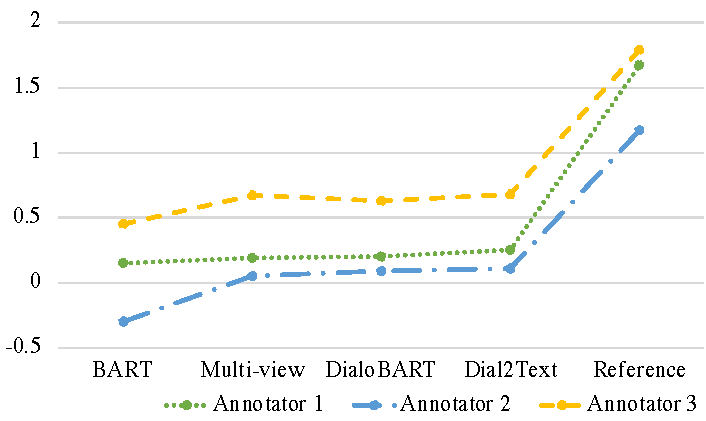
\includegraphics[scale=0.7]{humaneval.pdf}
	\caption{Trends of human evaluation scores for three annotators.}
	\label{fig:humaneval}
\end{figure}

%\begin{table}[h]
%	\centering
%	\small
%	\begin{tabular}{lccc}
%		\toprule[1pt]
%		\textbf{Models} & \textbf{Annotator 1} & \textbf{Annotator 2} & \textbf{Annotator 3} \\
%		\midrule[1pt]
%		BART & 0.15& -0.3&0.45\\
%		Multi-view & 0.19& 0.05&0.67 \\
%		DialoBART & 0.2& 0.09& 0.63\\
%		Dial2Text &\textbf{0.25} &\textbf{0.11} & \textbf{0.68}\\
%		\midrule[1pt]
%		Reference & 1.67& 1.17&1.79 \\
%		\bottomrule[1pt]
%	\end{tabular}
%	\caption{The overall scores from different annotators.}
%	\label{tab:annotator}
%\end{table}

%To further compare the performance of Dial2Text with Multi-view and DialoBART, we transform the scores into ``Better-Equal-Worse" by comparing original scores within each sample. The Fleiss Kappa is also 0.34 with fair agreement. The results in Table \ref{tab:betterworse} shown the competitive results of Dial2Text with the state-of-the-art methods. It should be noted that Dial2Text can be easily applied to other dialogue scenarios while others can't.

%\begin{table}[h]
%	\centering
%	\small
%	\begin{tabular}{lcc}
%		\toprule[1pt]
%		\textbf{Annotator} & \textbf{Comparison} & \textbf{Better-Equal-Worse} \\
%		\midrule[1pt]
%		\multirow{2}{1pt}{1} & Dial2Text v.s. Multi-view & 51-107-42 \\
%		& Dial2Text v.s. DialoBART & 51-101-48 \\
%		\multirow{2}{1pt}{2} & Dial2Text v.s. Multi-view & 32-137-31\\
%		& Dial2Text v.s. DialoBART &42-119-39 \\
%		\multirow{2}{1pt}{3} & Dial2Text v.s. Multi-view & 27-147-26\\
%		& Dial2Text v.s. DialoBART &34-136-30 \\
%		\bottomrule[1pt]
%	\end{tabular}
%	\caption{The comparisons from different annotators.}
%	\label{tab:betterworse}
%\end{table}

\begin{table}[h]
	\centering
	\small
	\begin{tabular}{l}
		\toprule[1pt]
		\textbf{Multi-view} \\
		\hline
		\textit{Topic View:} William: hey im making spaghetti William: could\\ you please buy some fresh tomatoes \textbf{$\mid$} William: pretty please :) \\Olivia: no problem dear :) William: and Beth? it wouldn't hurt\\ to have some chocolate for after the dinner :D Beth: I'm on it\\ :D \textbf{$\mid$}\\
		\textit{Stage View:} \textbf{$\mid$} William: hey im making spaghetti William: could\\you please buy some fresh tomatoes \textbf{$\mid$} William: pretty please :) \\Olivia: no problem dear :) \textbf{$\mid$} William: and Beth? it wouldn't hurt\\to have some chocolate for after the dinner :D \textbf{$\mid$} Beth: I'm on it\\:D\\
		\hline
		\textbf{DialoBART} \\
		\hline
		William : hey im making spaghetti \textbf{$\mid$} William : could you please\\buy some fresh tomatoes \textbf{$\mid$} William : pretty please \textbf{$\mid$} Olivia : no\\problem dear \textbf{$\mid$} William : and Beth ? it wouldn't hurt to have\\ some chocolate for after the dinner :D \textbf{$\mid$} Beth : I'm on it :D \\\textbf{\#KEY\#} Olivia Beth William hey im making spaghetti Beth it :D\\
		\bottomrule[1pt]
	\end{tabular}
	\caption{The annotated dialogue by Multi-view and DialoBART.}
	\label{tab:annodial}
\end{table}



The labeled dialogues, which are directly extracted from Multi-view's and DialoBART's released datasets are shown in Table \ref{tab:annodial}. ``$\mid$'' label for Multi-view refers to the topic transitions and state transitions for the same dialogue respectively. They both suffer from some wrong labels, such as the topic transition after the second utterance and the stage transition before the last utterance from Beth.  ``$\mid$'' in DialoBART just refers to the end of each utterance. It actually fails to identify any topic segments or redundancies in this dialogue. There are also meaningless keywords, such as ``hey'' and ``:D''.

They failed on such simple dialogues due to the following reasons. Firstly, these designed features are more focused on content selection by segmenting the dialogue into pieces, annotating the redundant pieces or highlighting keywords. They all ignore the coreference and reasoning features which are also important for dialogue summarization. Secondly, it's doubtful that whether the model can learn such labeling schemas well. Thirdly, these features are labeled with other labeling tools and human-designed rules, which may not be suitable for all cases, leading to error propagation from wrong labels to poor summaries.


\section{Dial2Text Performance on CRD3 Dataset}



We also did experiments on CRD3 dataset~\cite{rameshkumar2020storytelling}, which contains role-playing dialogues between multiple participants. The number of train/dev/test dialogues are 26232/3470/4541. There are around 478.97 words in each dialogue. The compression ratio of this dataset is 17.35\%, similar to DialSumm. The abstractiveness of CRD3 is much lower than other datasets reflected by the highest Rouge-2 with 23.45\% among these five summarization datasets. 


\begin{table}[h]
	\centering
	\small
	\begin{tabular}{lccc}
		\toprule[1pt]
		\textbf{Models} & \textbf{Rouge-1} & \textbf{Rouge-2} & \textbf{Rouge-L} \\
		\midrule[1pt]
		%\multicolumn{4}{l}{\textit{Average among References}}\\
		%\midrule[1pt]
		{Ext} &25.20 &\textbf{9.23} &22.20 \\
		{Abs} & 23.25&4.91 &21.41\\
		{BART} & \textbf{27.04}&8.38 &\textbf{23.99} \\
		{Dial2Text} &26.95 &8.37 &23.97  \\
		\bottomrule[1pt]
	\end{tabular}
	\caption{Results(\%) on CRD3 test set.}
	\label{tab:crd3results}
\end{table}
Results on the CRD3 test set are shown in Table \ref{tab:crd3results}. Ext and Abs represent the extractive and abstractive baselines proposed by Rameshkumar and Bailey~\shortcite{rameshkumar2020storytelling}, which are derived from Fast-Abs~\cite{chen2018fast}.
The extractive baseline performs much better than the abstractive one, also reflecting the high extractiveness of this dataset. 
BART and our proposed Dial2Text exceed both baselines while performances on BART and Dial2Text are similar to each other without significant differences according to t-test.
It shows that our proposed approach is more suitable for more abstractive dialogue summarization tasks. At the same time, our post-training process didn't hurt the ability of the model on extractive datasets. 


An example is shown in Table~\ref{tab:crd3case}.
Since the paired dialogues and reference summaries in CRD3 are constructed by splitting the original long transcripts and episode summaries into segments. The reference summary tends to contain broken coreference chains and unaligned contents. For example, the reference in Table~\ref{tab:crd3case} starts with ``she'' while we can't figure out who she is barely based on the reference summary. The last sentence in the reference is also not mentioned in the given dialogue. 

In this dialogue, Sam Riegel~\footnote{\url{https://criticalrole.fandom.com/wiki/Sam_Riegel}} is an actor playing Scanlan Shorthalt and Taryon Darrington in the first campaign, and Veth Brenattor in the second campaign for ``Dungeons and Dragons'' role-playing games. As a result, both ``SAM'' and ``she'' in this sample should refer to ``Veth Brenattor''. Bart and Dial2Text mistake ``SAM'' to ``Scanlan''. The reason is that the training data for this corpus mainly constructed from the first campaign. Both models identify the relationship between the actor and the character during training, while this knowledge is not applicable for testing samples. This also leads to gender errors in both generated summaries.

The generated summaries are similar to each other with close rouge scores. In this sample, Bart acted like selecting the key utterance and simply replacing the subject ``I'' with speaker names. Dial2Text tried to integrate more contexts such as ``gold'' and rephrase the sequence of ``and'' utterance into more formal expressions, but also introduced errors.

\begin{table}
	\centering
	\small
	\begin{tabular}{p{1.2cm}p{6cm}}
		\toprule[1pt]
		Dialogue &\makecell[l]{SAM: To buy a bunch of baubles and trinkets \\\quad\quad\quad and buttons and ribbons and string and \\\quad\quad\quad beads and one crescent ornament. \\
			MATT: Okay, I will say you could purchase all \\\quad\quad\quad of those things-- and you're buying these \\\quad\quad\quad yourself? \\
			SAM: In Disguise Self mode. \\
			MATT: Okay, yeah. I'd say you could buy all of \\\quad\quad\quad those things with, let's say, a single gold, \\\quad\quad\quad because your charisma isn't that high. A \\\quad\quad\quad single gold piece for all of that. That's \\\quad\quad\quad priced up a bit. \\
			SAM: That's pretty good. \\\quad\quad\quad LAURA: That's pretty \\\quad\quad\quad good. \\
			SAM: I will put all of that stuff into a package \\\quad\quad\quad and mail it away with a note that I sent \\\quad\quad\quad you earlier, Matt.\\
		}\\
		\hline
		Reference & She puts it all in a package with a note and 100 gp, and mails the package to a yet-to-be-revealed location. She also buys tinkerer's tools for 50 gp.\\
		\hline
		BART &  Scanlan buys a bunch of baubles and trinkets and buttons and ribbons and string and beads and one crescent ornament. He puts all of that stuff into a package and mail it away with a note that he sent to Matt. \textbf{(37.14/8.82/32.73)}\\
		\hline
		Dial2Text &   Scanlan spends a bunch of gold on baubles, ribbons, string, beads, and one crescent ornament. He puts all of that stuff into a package and sends it away with a note that he sent to Matt earlier. \textbf{(36.36/9.37/28.57)}\\
		\bottomrule[1pt]
	\end{tabular}	
	\caption{An example from CRD3 dataset}
	\label{tab:crd3case}  	
\end{table}



\section{Case Studies}

We show more cases from DialSumm, Email and TopicAMI in Table~\ref{tab:dialsummcase1}, Table~\ref{tab:emailcase1} and Table~\ref{tab:topicamicase1}. Dialogues display in these tables are the original ones from corresponding datasets without additional labels.

Dialogues from DialSumm are similar to dialogues from SAMSum, but more challenging with higher abstractiveness, more formal style and more diverse task-oriented topics~\cite{chen2021dialsumm}. By analyzing the generated results, we also find that the normalization for speaker names like ``\#Person1\#'' in DialSumm brings obstacles for understanding and reasoning in summarization. The model is not only required to figure out the coreference relations between pronouns, such as I and you, and speakers, but also infer the names of speakers if mentioned in the dialogue. Examples in Table~\ref{tab:dialsummcase1} show that Dial2Text can do reasoning and coreference resolution better than other approaches with less unfaithful contents.

Table~\ref{tab:emailcase1} exemplifies the generated summaries by BART and Dial2Text from Email. Our approach tends to merge the contents from the same person.  Dialogue summarization for e-mail threads is much more difficult with inherent structures including sender, receivers, a subject and body texts. In this paper, we follow the previous paper~\cite{fabbri2021convosumm} by concatenating all of the e-mails into a single input sequence for models, and try to provide a general post-trained model for dialogue summarization tasks with strong generalization ability.

Summaries in TopicAMI are close to categorical high-level topic descriptions. We show two extreme cases in Table~\ref{tab:topicamicase1}. BART and Dial2Text both succeed on the first case and fail on the other one. For the second case, ``chitchat'' generated by Dial2Text is closer to ``opening'' semantically. This dialogue is difficult for too many colloquial words without clear meanings, such as ``yep'' and ``mm-hmm''. Higher overall rouge scores on this dataset also support that our post-trained model does narrow the understanding gap from dialogue to narrative text, providing a better initial state for downstream fine-tuning than BART on cross-format tasks.




\begin{table*}
	\centering
	\small
	\begin{tabular}{p{1.5cm}p{14.5cm}}
		\toprule[1pt]
		
		Dialogue & \makecell[l]{\#Person1\#: Maggie, can I borrow your notes for history? I'll return them tomorrow.\\
		\#Person2\#: Sorry, but I usually go to the cafeteria and review them. Why not copy them in the library?\\
		\#Person1\#: OK.\\
		\#Person2\#: Here you are.\\
		\#Person1\#: You are a great help, Maggie.\\
		\#Person2\#: I don't quite understand a why you need my notes, Mark? You haven't missed any classes.\\
		\#Person1\#: To be honest, I work in supermarket from 7 to 10 o'clock every evening.\\
		\#Person2\#: I see. So you're pretty tired when you come to class.\\
		\#Person1\#: That's exactly why I want to borrow your notes. My notes aren't very good.\\
		\#Person2\#: So what do you usually do in class?\\
		\#Person1\#: I'm always awake at the beginning, but thirty minutes after class begins I feel sleepy and have trouble \\\quad\quad\quad\quad\quad keeping my eyes open.\\
		\#Person2\#: Well, I need someone to study with and you need someone to keep you awake. Can we be study\\ \quad\quad\quad\quad\quad partners?\\
		\#Person1\#: Oh sure. That's a good idea. So give me a push when you see me sleeping in class.\\
		\#Person2\#: OK. Let's start today in the library. We are going there anyway and I don't have to go to the cafeteria.\\
		\#Person1\#: Sounds good.}\\
		\hline
		Reference\-1 & Mark wants to borrow Maggie's class notes. Maggie suggests Mark copy them in the library and invites him to be study partners. \\
				\hline
		Reference\-2 & Mark asks Maggie for her history notes because Mark has been too tired in class. They become study partners at the end. \\
				\hline
		Reference\-3 & Mark asks Maggie for her notes because Mark's notes aren't good. They decide to be study partners and study together. \\
				\hline
		DialoBART & \textit{Mark} borrows Maggie's notes for history and \textit{asks her to be study partners}. \textit{Maggie} tells Mark that she usually goes to the cafeteria to review the notes but \textit{she feels sleepy and has trouble keeping her eyes open}. \textit{Mark suggests copying them in the library}. \textbf{(Avg: 41.16/19.49/38.78 Max:47.76/36.92/47.27)}\\
				\hline
		Multi-view & Mark wants to borrow Maggie's notes because his notes aren't very good and \textit{he feels sleepy after class}. Maggie suggests copying them in the library and they will be study partners to \textit{keep each other awake}. \textbf{(Avg: 45.32/29.76/44.29 Max: 62.07/42.86/60.38)}\\
				\hline
		BART & Mark wants to borrow Maggie's notes for history. \textit{Maggie refuses because she usually copies them in the cafeteria}. Then they talk about what they usually do in class and decide to be study partners. \textbf{(Avg: 45.72/27.16/46.65 Max:57.14/40.74/60.00)}\\
				\hline
		Dial2Text & Mark wants to borrow Maggie's notes for history because he feels sleepy after class begins. Maggie suggests copying them in the library and they will be study partners. \textbf{(Avg: 51.22/30.56/48.36 Max: 68.00/45.83/66.67)}\\
		\midrule[1pt]
		Dialogue & \makecell[l]{\#Person1\#: What can I do for you?\\
		\#Person2\#: I want to get my car washed.\\
		\#Person1\#: Would you like regular car wash package?\\
		\#Person2\#: I don't know what you mean.\\
		\#Person1\#: Well, we will wash the exterior form top to bottom. We use a special shampoo, which gives the body \\ \quad\quad\quad\quad\quad that extra shine.\\
		\#Person2\#: Do you wash windows?\\
		\#Person1\#: Of course. We wash the windows inside and out.\\
		\#Person2\#: What about the interior?\\
		\#Person1\#: We use a vacuum cleaner that removes all the dirt, and we throw away all of the trash that we can find.\\
		\#Person2\#: Sounds good, regular car wash package will be OK.\\
		\#Person1\#: OK. I see.} \\
		\hline
		References1&  \#Person1\# describes the contents of the regular car wash package. \#Person2\# will take that.\\
		\hline
		References2&  \#Person1\# introduces the content of regular car wash package and \#Person2\# accepts.\\
		\hline
		References3&  \#Person1\# introduces the services included in regular car wash package and \#Person2\# will take it.\\
		\hline
		DialoBART&  \#Person2\# wants to get \textit{\#Person1\#'s car} washed. \textbf{(Avg: 19.43/6.06/16.24 Max: 21.05/18.18/20.00)}\\
		\hline
		Multi-view&  \#Person1\# tells \#Person2\# how to wash the exterior and interior of the car with a regular car wash package. \textbf{(Avg: 53.22/31.18/50.74 Max:58.06/47.06/55.17)}\\
		\hline
		BART&  \#\#Person1\# tells \#Person2\# how to get the car washed. \textbf{(Avg: 26.55/8.33/23.77 Max: 28.57/25.00/27.27)}\\		
		\hline
		Dial2text& \#Person2\# wants to get his car washed. \#Person1\# recommends a regular car wash package. \textbf{(Avg: 43.46/29.82/45.18 Max: 46.15/41.37/48.00)}\\
		
		\bottomrule[1pt]
	\end{tabular}
	
	\caption{Examples from DialSumm. \textit{Unfaithful contents} are italicized. Rouge-1/2/L scores(\%) are appended in parentheses.}
	\label{tab:dialsummcase1}  
\end{table*}


\begin{table*}
	\centering
	\small
	\begin{tabular}{p{1.5cm}p{14.5cm}}
		\toprule[1pt]
		Emails & Name: ``Nilo Mitra (EUS)''   Email: ``Nilo.Mitra@am1.ericsson.se''   To: ``Nilo Mitra (EUS)''$\langle$Nilo.Mitra@am1.ericsson.se$\rangle$,``Jean-Jacques Moreau‘’$\langle$moreau@crf.canon.fr$\rangle$,``Martin Gudgin‘’$\langle$mgudgin@microsoft.com$\rangle$,``Marc Hadley''$\langle$marc.hadley@sun.com$\rangle$,``Noah Mendelson''$\langle$noah\_mendelsohn@us.ibm.com$\rangle$,``Henrik Frystyk Nielsen''$\langle$henrikn@microsoft.com$\rangle$   Subject: ``Is LC issue 309 misdirected at Primer?''            Gentlemen:   Might perhaps LC issue 309 [1] be a more general matter, and misdirected at Part0: Primer by mistake? (The remainder of the originator's comments are on the Primer, from which this one is an excerpt.)   Please clarify,   Thanks   Nilo   [1] http://www.w3.org/2000/xp/Group/xmlp-lc-issues.html\#x309              $\langle$/s$\rangle$Name: ``Martin Gudgin''   Email: ``mgudgin@microsoft.com''   To: Nilo Mitra (EUS); 'Jean-Jacques Moreau'; Martin Gudgin; 'Marc   Subject: ``RE: Is LC issue 309 misdirected at Primer?''            I agree this is a comment on the spec in general. It is also a dupe ( of   Issue 277[2] )       Gudge       [2] http://www.w3.org/2000/xp/Group/xmlp-lc-issues.html\#x277    $\langle$/s$\rangle$Name: ``Nilo Mitra (EUS)''   Email: ``Nilo.Mitra@am1.ericsson.se''   To: Nilo Mitra (EUS); 'Jean-Jacques Moreau'; Martin Gudgin; 'Marc Hadley'; 'Noah Mendelson'; Henrik Frystyk Nielsen   Subject: ``RE: Is LC issue 309 misdirected at Primer?''            Could the resolution of Issue 333 [3] have a bearing on the handling of this issue?   Nilo   [3] http://www.w3.org/2000/xp/Group/xmlp-lc-issues.html\#x333 <http://www.w3.org/2000/xp/Group/xmlp-lc-issues.html\#x333>              $\langle$/s$\rangle$Name: ``Martin Gudgin''   Email: ``mgudgin@microsoft.com''   To: Nilo Mitra (EUS); 'Jean-Jacques Moreau'; Martin Gudgin; 'Marc   Subject: ``RE: Is LC issue 309 misdirected at Primer?''            Agreed, so 227 is a dupe too ;-)       Gudge\\
		\hline
		Reference & Nilo asks if LC issue 309, which addresses Part0: Primer, is a more general issue. Martin agrees and notes that it’s a duplicate of issue 277. Nilo then wonders if the resolution to issue 333 affects this issue. Martin agrees and says that 227 is also a duplicate.\\
		\hline
		BART & Nilo Mitra asks if LC issue 309 misdirected at Primer by mistake. Martin Gudgin replies that it is a comment on the spec in general. Henrik Frystyk Nielsen asks if the resolution of Issue 333 has a bearing on the handling of this issue. Marc Hadley replies that Issue 333 is a dupe. \textbf{(41.58/14.14/41.10)}\\
		\hline
		Dial2Text & Nilo Mitra asks if LC issue 309 is misdirected at Primer or if Issue 333 has a bearing on the handling of this issue. Martin Gudgin agrees that Issue 277 is a duplicate of Issue 309 and agrees that 227 is also a dupe. \textbf{(56.52/26.67/51.52)}\\		
		\bottomrule[1pt]
	\end{tabular}

	\caption{An example from Email. $\langle$/s$\rangle$ is the separator between e-mails.}
	\label{tab:emailcase1}  
\end{table*}

\begin{table*}
	\centering
	\small
	\begin{tabular}{p{1.5cm}p{14.5cm}}
		\toprule[1pt]
		
		Dialogue &it makes it twelve , yeah . $\langle$EOS$\rangle$ yeah . $\langle$EOS$\rangle$ s $\langle$EOS$\rangle$ indeed . okay . $\langle$EOS$\rangle$ well , $\langle$EOS$\rangle$ not really $\langle$EOS$\rangle$ and $\langle$EOS$\rangle$ and there are some models that don't uh accommodate that function . $\langle$EOS$\rangle$ so $\langle$EOS$\rangle$ d uh wh $\langle$EOS$\rangle$ the philip's television makes it possible in that indeed to uh press one and then two to make uh the uh tj to reach channel twelve . $\langle$EOS$\rangle$ but uh all the television makes uh use of those button where you first press that button and then press two digits to uh to get $\langle$EOS$\rangle$\\
		\hline
		Reference &  look and usability\\
		\hline
		BART &  look and usability \textbf{(100/100/100)}\\
		\hline
		Dial2Text &  look and usability \textbf{(100/100/100)}\\
		\midrule[1pt]
		
		Dialogue &yeah . $\langle$EOS$\rangle$ and do you think it's . $\langle$EOS$\rangle$ yep . $\langle$EOS$\rangle$ okay . $\langle$EOS$\rangle$ yeah . $\langle$EOS$\rangle$ jo's making faces at me . $\langle$EOS$\rangle$  yeah . $\langle$EOS$\rangle$  so . $\langle$EOS$\rangle$  matthew is uh late again . $\langle$EOS$\rangle$  mm-hmm . $\langle$EOS$\rangle$  probably an important man . $\langle$EOS$\rangle$  um . so well $\langle$EOS$\rangle$  it is important for him to be here uh . $\langle$EOS$\rangle$ \\
		\hline
		Reference &opening \\
		\hline
		BART & drawing exercise \textbf{(0.0/0.0/0.0)}\\
		\hline
		Dial2Text & chitchat \textbf{(0.0/0.0/0.0)}\\
		\bottomrule[1pt]
	\end{tabular}
	
	\caption{Examples from TopicAMI. $\langle$EOS$\rangle$ represents the end of each utterance.}
	\label{tab:topicamicase1}  
\end{table*}


\bibliography{aaai22}

\end{document}
